%%%%%%%%%%%%%%%%%%%%%%%%%%%%%%%%%%%%%%%%%%%%%%%%%%%%%%%%%%%%%%%%%%
%%%%%%%% ICML 2014 EXAMPLE LATEX SUBMISSION FILE %%%%%%%%%%%%%%%%%
%%%%%%%%%%%%%%%%%%%%%%%%%%%%%%%%%%%%%%%%%%%%%%%%%%%%%%%%%%%%%%%%%%

% Use the following line _only_ if you're still using LaTeX 2.09.
%\documentstyle[icml2014,epsf,natbib]{article}
% If you rely on Latex2e packages, like most moden people use this:
\documentclass{article}

% use Times
\usepackage{times}
% For figures
\usepackage{graphicx} % more modern
%\usepackage{epsfig} % less modern
\usepackage{subfigure} 

% For citations
\usepackage{natbib}

% For algorithms
\usepackage{algorithm}
\usepackage{algorithmic}

% As of 2011, we use the hyperref package to produce hyperlinks in the
% resulting PDF.  If this breaks your system, please commend out the
% following usepackage line and replace \usepackage{icml2014} with
% \usepackage[nohyperref]{icml2014} above.
\usepackage{hyperref}

% Packages hyperref and algorithmic misbehave sometimes.  We can fix
% this with the following command.
\newcommand{\theHalgorithm}{\arabic{algorithm}}

% Employ the following version of the ``usepackage'' statement for
% submitting the draft version of the paper for review.  This will set
% the note in the first column to ``Under review.  Do not distribute.''
%\usepackage{icml2014} 
% Employ this version of the ``usepackage'' statement after the paper has
% been accepted, when creating the final version.  This will set the
% note in the first column to ``Proceedings of the...''
\usepackage[accepted]{icml2014}


% The \icmltitle you define below is probably too long as a header.
% Therefore, a short form for the running title is supplied here:
\icmltitlerunning{Graphical models: Structure learning}

\begin{document} 

\twocolumn[
\icmltitle{Graphical models: Structure learning \\
						Hauptseminar Machine learning, WS 13/14}

% It is OKAY to include author information, even for blind
% submissions: the style file will automatically remove it for you
% unless you've provided the [accepted] option to the icml2014
% package.
\icmlauthor{Moritz Hamann}{moritz.hamann@gmx.com}
\icmladdress{University of Stuttgart}


% You may provide any keywords that you 
% find helpful for describing your paper; these are used to populate 
% the "keywords" metadata in the PDF but will not be shown in the document
\icmlkeywords{graphical models, structure learning, bayesian networks, full bayesian approach}

\vskip 0.3in
]

\begin{abstract} 
Super cool abstract
\end{abstract} 


\section{Introduction}
The goal of this paper is to present the main ideas of [ref], which describes[?] a Bayesian approach
for structure learning of Bayesian networks. Furthermore, we'll show the contribution of the author to
the relevant field, as well as provide additional experimental results, which we conducted on our own.

warum structure learning - bayesian approach - vorteile fuer sample likelihood

\section{Related research}
anderes paper gleicher author - neue papers researchen

\section{Basics}
In this chapter, we present the basics

	\subsection{Bayesian network}
	A Bayesian network (sometimes also called a Bayes or belief network) is a probabilistic graphical model
	which encodes the conditional dependencies between a set of random variables (RV) $X=\{X_1,..., X_n\}$.
	Such a network	is a Directed Acyclic Graph (DAG), which nodes represent the RV, and the edges 
	describe the conditional
	dependencies between these RV. Therefore, each node in the Bayesian network can be seen as a 
	conditional probability distribution of the random variable $X_i$ under its parents $Pa_i$.
	This would result in $P(X_i|Pa_i)$. ?????
	
	Figure[ref] shows a simple Bayesian network with three binary random variables, and
	the CPT for $X_3$.	
	 
	\subsection{Dirichlet probability distribution}
	The Dirichlet distribution is a multivariate continuous probability distribution, which depend on a
	vector $\alpha$ with positive entries. It is defined as
	\[
		Dir(x_1,...,x_m|\alpha_1, ..., \alpha_{m})=\frac{1}{B(\alpha)}\prod_{i=1}^m x_i^{\alpha_i -1}
	\]
	where $\sum_i x_i = 1$, $x_i>0$ and 
	\[
		B(\alpha)=\frac{\prod_{i=1}^m\Gamma(\alpha_i)}{\Gamma(\sum_{i=1}^m \alpha_i)}
	\]
	with the Gamma function $\Gamma(x)$. Since $B(\alpha)$ is the multinomial extension of the Beta function,
	the Dirichlet distribution can be seen as the	multivariate generalization of the Beta distribution.
	[[ Note that equal a is uniform distribution and what ai stands for, and equivalent sample size + ref]]
	
	The Dirichlet distribution is also the conjugated prior of the multinomial distribution.
	Therefore, it is often used in Bayesian probability theory to model the belief $P(\mu)$ about the
	parameter of a multinomial distribution $Multi(x|\mu)$ for a discrete random variable $x$.
	This yields the benefit of a simple calculation of the posterior $P(\mu|x)$. If x corresponds to
	a dataset $D$ which contains
	Therefore, the posterior $P(\mu|D)$ is also Dirichlet distributed and is given by
	\[
		P(\mu|D) \propto Dir(\mu|\alpha_1+n_1, ..., \alpha_k+n_k)
	\]	
	where $\alpha_i$ is from the prior and $n_i$ the number of occurences in D...
	For detailed information about the Dirichlet distribution, as well as the calculation of the
	posterior, we refer to[ref].

\section{Structure learning}
	In order to learn the model of a Bayesian network 
	from an observed dataset $D=\{d_1,...,d_N\}$ where $d_i$ is a full observation of $X$,
	the authors of [ref]	proposed a Bayesian approach 
	and introduced the random variable $m$. It has the states $m_1,...m_M$ which correspond to the 
	possible models of a Bayesian network for the set of random variables $X$.
	
	\subsection{Assumption}
	The authors of [ref] considered discrete random variables for $X$, which means	every $X_i$ has a
	finite number of	states $r_i$. We use the notation $x_i^k$ if the random variable $X_i$ is in state $k$
	with $k = 1...r_i$. Since every $X_i$ has a finite number of parents $Pa_i$, there exists
	a finite amount of possible combinations for the parents states $q_i=\prod_{X_m \in Pa_i} r_m$.
	We denote a specific configuration $j$ of $Pa_i$ with $pa_i^j$ and $j=1...q_i$. 
	
	In addition	to discrete random variables, the authors also assumed that the state of $X_i$ with a specific
	parent state combination $pa_i^j$ is multinomial distributed with a parameter vector $\theta_{ij}$.
	
	This simplifies the construction and inference in the Bayesian network,	because the probability
  distribution for each node can now be stored as a conditional probability table (CPT). In this CPT
	exists a parameter vector $\theta_{ij}$ for every random variable and every possible parent state
	combination. To denote the probability for a state $k$ of $X_i$ with parent state $pa_i^j$, we
	use the notation $\theta_{ijk}$. Since the states of $X_i$ are multinomial distributed it is clear
	that
	\[
		\sum_{k=1}^{r_i} \theta_{ijk} = 1
	\]
	In the following sections we refer to the full set of parameters as $\theta^m$ for a specific.	
	
	\subsection{Bayesian approach}
	In order to find the optimal model $m$ for an observation $D$, one has to maximize the posterior of $m$
	under $D$. Using the Bayes' rules this yields 
	\[
		P(m|D) = \frac{P(D|m)P(m)}{P(D)}=\frac{P(D|m)P(m)}{\sum_m P(D|m)P(m)}
	\]
	for the posterior of $m$. Similar, one can compute the posterior for the parameter set $\theta^m$ dependent
	on the observed data
	\[
		P(\theta^m|D,m)= \frac{P(D|\theta^m,m)P(\theta^m|m)}{p(D|m)}
	\]
	In both equations it is necessary to compute the likelihood of the dataset $D$ under a specific model $m$.
	The authors refer to it as the \textit{marginal likelihood}, which is given as an integral over all
	possible values for $\theta^m$
	\[
		P(D|m) = \int P(D|\theta^m,m)P(\theta^m|m) d\theta^m
	\]
	Before going into detail how to calculate the marginal likelihood, or how to choose the model and parameter
	priors, we want to focus on the benefits of the Bayesian approach as pointed out by the authors. In
	contrast to other methods [[ find references ]], which learn only the most probable model, the
	Bayesian approach yields a probability distribution over all possible models. This allows a 
	comparison of the probability between different models or the selection of models which have a similar
	probability than the best.
	
	Another important benefit is the ability to determine the probability of a hypothesis,
	i.e. the likelihood of a	new data sample $d_{N+1}$, over all possible models
	instead on only the most likely one. The probability of the new data sample is then
	\[
		P(d_{N+1}|D)=\sum_m P(m|D)\int P(d_{N+1}|\theta^m,m)P(\theta^m|m)d\theta^m
	\]
	The author call these a \textit{full} Bayesian approach, since the probability is determined as an average
	over all possible models. Unfortunately, the number of possible models in a DAG with $n$ nodes grows
	super exponentially with $n$. Therefore, the averaging over all possible models is impractical and
	one often chooses a fixed number of the most likely models and pretend that these are exhaustive.
	
	\subsection{Model prior}
	The most simple choice for the model prior $P(m)$ is a uniform distribution. This represents 
	the belief that no information about the model structure is	available and thus every 
	model is same likely. If some information about the problem domain are available, the search space 
	of models can be reduced by excluding specific models or model families (e.g. if some random
	variables cant have parents or children). This is achieved by setting
	the prior $P(m)$ for these model to zero and assume an uniform distribution over the remaining
	models.	
	
	An other possibility for the choice of the model prior, as mentioned by the authors, is given
	by Buntine [ref]. In this case the prior distribution can be computed under the assumption that
	the random variables can be ordered (e.g. through time precedence). For detailed information we
	refer to the original paper [ref].
	
	\subsection{Parameter prior}
	Another important choice is the prior distribution for the parameters $P(\theta^m|m)$. To simplify
	the computation the authors assumed parameter independence, which means that the joint probability
	distribution can be computed with
	\[
		P(\theta^m|m)= \prod_{i=1}^n \prod_{j=1}^{q_i} P(\theta_{ij}|m)
	\]
	The parameter independence also holds for the posterior $P(\theta_{ij}|D,m)$, which means
	that each $\theta_{ij}$ can be updated individually.
	
	As mentioned before, a common choice in Bayesian probability theory for unknown parameter distributions
	is to use the conjugated prior distribution of the likelihood.
	Since the authors assumed a multinomial distribution
	for $X_i$, the likelihood $P(D|\theta_{ij},m)$ is also multinomial distributed, and hence the
	conjugated prior would be the Dirichlet distribution
	\[
		P(\theta_{ij}|m) = Dir(\theta_{ij}|\alpha)
	\]
	with $\alpha_i > 0$.
	
	An important contribution of the authors is the proof that certain assumptions actually 
	imply a Dirichlet distribution of the parameter prior $P(\theta^m|m)$.
	The complete proof, as well as detailed information on these assumptions, is given in [ref].
	The following section briefly presents three key concepts of the proof.
	
	\textbf{Markov equivalence:}
	Two models $m_1$ and $m_2$ for a set of random variables $X$ are called \textit{markov equivalent},
	if they encode the same conditional independence relation (?) of $X$. For example, in the case of
	$X=\{X_1,X_2,X_3\}$, the models $X_1 \rightarrow X_2 \rightarrow X_3$,
	$X_1 \leftarrow X_2 \leftarrow X_3$ and $X_1 \leftarrow X_2 \rightarrow X_3$ are 
	markov equivalent, since they all encode that $X_1$ and $X_3$ are independent, given $X_2$.
	As shown by the authors, the set of complete models for $X$ is also markov equivalent. 
	A complete model is a DAG in which every $X_i$ has either an 	incoming or outgoing edge 
	to every other $X_j$. [[ brauchen wir das?]]
	
	\textbf{Distribution equivalence:}
	Two models $m_1$ and $m_2$ are called \textit{distribution equivalent} (with respect to some distribution
	family $\mathcal{F}$), if they represent the same
	joint probability distribution. This is the case, if for every $\theta^{m_1}$ exists a $\theta^{m_2}$
	so that $P(x|\theta^{m_1},m_1) = P(x|\theta^{m_2},m_2)$. Distribution equivalence is closely related
	to markov equivalence, and in fact, distribution equivalence implies markov equivalence, where the
	opposite may not hold. [[ data instead of x? ]]
	
	\textbf{Parameter modularity:}
	The assumption of \textit{parameter modularity} implies that $P(\theta_{ij}|m_1) = P(\theta_{ij}|m_2)$
	if the random variable $X_i$ has the same parents in the model $m_1$ and $m_2$. [[genauer?]]
	
	The authors argued that if two models are distribution equivalent, it is unlikely that data can
	discriminate them. Therefore they assumed $P(D|m_1)=P(D|m_2)$ and called this
	property \textit{likelihood equivalence}.
	Under the assumption of likelihood equivalence, and	parameter independence, the authors were able to
	show that the parameters of every complete model have to be Dirichlet distributed. Together we
	the assumption of parameter modularity, this implies a Dirichlet distribution even for non-complete
	models. [[ man kann immer complete model construieren in dem parents wie im incomplete sind ]]
	
	\subsection{Computation of the marginal likelihood}
	As shown in section [ref] the computation of the model posterior distribution depends on the model prior,
	which was addressed in section [ref],	as well as the marginal likelihood. Eqn [ref] shows it
	as the integral over all possible
	
	closed loop evaluation 
	
	

\section{Heuristics}
\section{evaluation results}

\section{relevance}

\section{conclusion}





%--------------------------------------------------------




 
You can use footnotes\footnote{For the sake of readability, footnotes
should be complete sentences.} to provide readers with additional
information about a topic without interrupting the flow of the paper. 
Indicate footnotes with a number in the text where the point is most
relevant. Place the footnote in 9~point type at the bottom of the
column in which it appears. Precede the first footnote in a column
with a horizontal rule of 0.8~inches.\footnote{Multiple footnotes can
appear in each column, in the same order as they appear in the text,
but spread them across columns and pages if possible.}

\begin{figure}[ht]
\vskip 0.2in
\begin{center}
\centerline{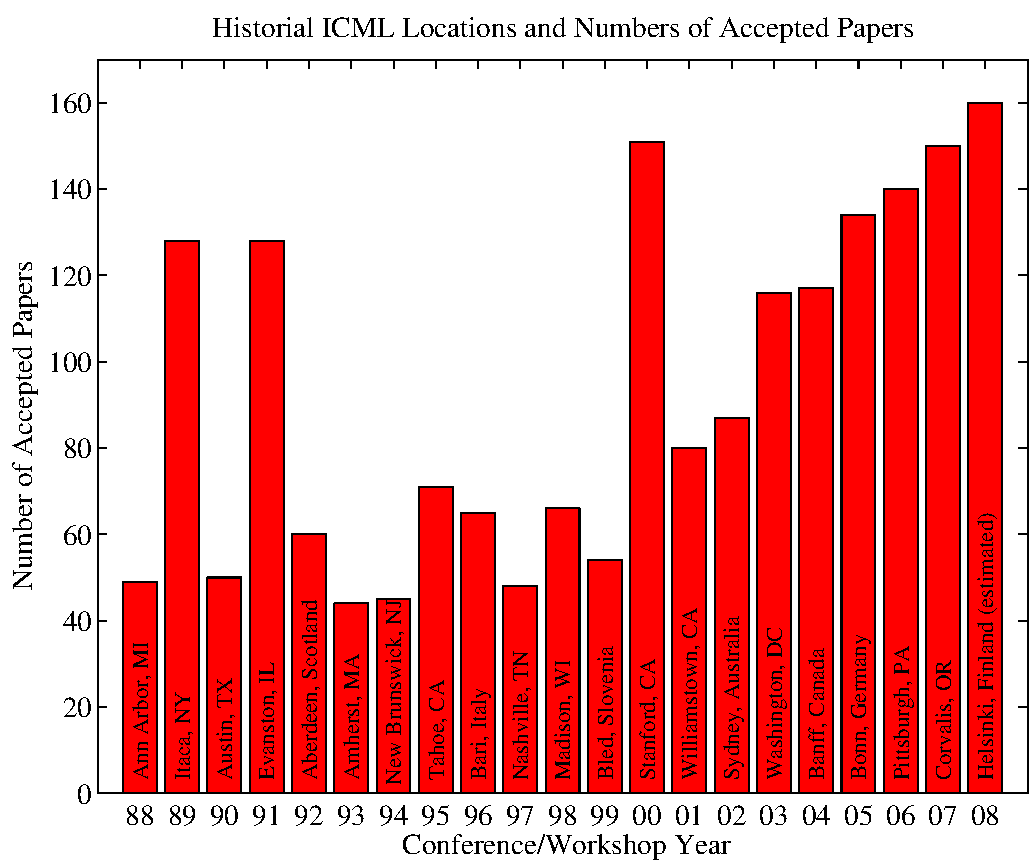
\includegraphics[width=\columnwidth]{icml_numpapers}}
\caption{Historical locations and number of accepted papers for International
  Machine Learning Conferences (ICML 1993 -- ICML 2008) and
  International Workshops on Machine Learning (ML 1988 -- ML
  1992). At the time this figure was produced, the number of
  accepted papers for ICML 2008 was unknown and instead estimated.}
\label{icml-historical}
\end{center}
\vskip -0.2in
\end{figure} 

\subsection{Figures}
 
You may want to include figures in the paper to help readers visualize
your approach and your results. Such artwork should be centered,
legible, and separated from the text. Lines should be dark and at
least 0.5~points thick for purposes of reproduction, and text should
not appear on a gray background.

Label all distinct components of each figure. If the figure takes the
form of a graph, then give a name for each axis and include a legend
that briefly describes each curve. Do not include a title inside the
figure; instead, the caption should serve this function.

Number figures sequentially, placing the figure number and caption
{\it after\/} the graphics, with at least 0.1~inches of space before
the caption and 0.1~inches after it, as in
Figure~\ref{icml-historical}.  The figure caption should be set in
9~point type and centered unless it runs two or more lines, in which
case it should be flush left.  You may float figures to the top or
bottom of a column, and you may set wide figures across both columns
(use the environment {\tt figure*} in \LaTeX), but always place
two-column figures at the top or bottom of the page.

\subsection{Algorithms}

If you are using \LaTeX, please use the ``algorithm'' and ``algorithmic'' 
environments to format pseudocode. These require 
the corresponding stylefiles, algorithm.sty and 
algorithmic.sty, which are supplied with this package. 
Algorithm~\ref{alg:example} shows an example. 

\begin{algorithm}[tb]
   \caption{Bubble Sort}
   \label{alg:example}
\begin{algorithmic}
   \STATE {\bfseries Input:} data $x_i$, size $m$
   \REPEAT
   \STATE Initialize $noChange = true$.
   \FOR{$i=1$ {\bfseries to} $m-1$}
   \IF{$x_i > x_{i+1}$} 
   \STATE Swap $x_i$ and $x_{i+1}$
   \STATE $noChange = false$
   \ENDIF
   \ENDFOR
   \UNTIL{$noChange$ is $true$}
\end{algorithmic}
\end{algorithm}
 
\subsection{Tables} 
 
You may also want to include tables that summarize material. Like 
figures, these should be centered, legible, and numbered consecutively. 
However, place the title {\it above\/} the table with at least 
0.1~inches of space before the title and the same after it, as in 
Table~\ref{sample-table}. The table title should be set in 9~point 
type and centered unless it runs two or more lines, in which case it
should be flush left.

% Note use of \abovespace and \belowspace to get reasonable spacing 
% above and below tabular lines. 

\begin{table}[t]
\caption{Classification accuracies for naive Bayes and flexible 
Bayes on various data sets.}
\label{sample-table}
\vskip 0.15in
\begin{center}
\begin{small}
\begin{sc}
\begin{tabular}{lcccr}
\hline
\abovespace\belowspace
Data set & Naive & Flexible & Better? \\
\hline
\abovespace
Breast    & 95.9$\pm$ 0.2& 96.7$\pm$ 0.2& $\surd$ \\
Cleveland & 83.3$\pm$ 0.6& 80.0$\pm$ 0.6& $\times$\\
Glass2    & 61.9$\pm$ 1.4& 83.8$\pm$ 0.7& $\surd$ \\
Credit    & 74.8$\pm$ 0.5& 78.3$\pm$ 0.6&         \\
Horse     & 73.3$\pm$ 0.9& 69.7$\pm$ 1.0& $\times$\\
Meta      & 67.1$\pm$ 0.6& 76.5$\pm$ 0.5& $\surd$ \\
Pima      & 75.1$\pm$ 0.6& 73.9$\pm$ 0.5&         \\
\belowspace
Vehicle   & 44.9$\pm$ 0.6& 61.5$\pm$ 0.4& $\surd$ \\
\hline
\end{tabular}
\end{sc}
\end{small}
\end{center}
\vskip -0.1in
\end{table}

\subsection{Citations and References} 

Please use APA reference format regardless of your formatter
or word processor. If you rely on the \LaTeX\/ bibliographic 
facility, use {\tt natbib.sty} and {\tt icml2014.bst} 
included in the style-file package to obtain this format.

Citations within the text should include the authors' last names and
year. If the authors' names are included in the sentence, place only
the year in parentheses, for example when referencing Arthur Samuel's
pioneering work \yrcite{Samuel59}. Otherwise place the entire
reference in parentheses with the authors and year separated by a
comma \cite{Samuel59}. List multiple references separated by
semicolons \cite{kearns89,Samuel59,mitchell80}. Use the `et~al.'
construct only for citations with three or more authors or after
listing all authors to a publication in an earlier reference \cite{MachineLearningI}.

Authors should cite their own work in the third person
in the initial version of their paper submitted for blind review.
Please refer to Section~\ref{author info} for detailed instructions on how to
cite your own papers.

Use an unnumbered first-level section heading for the references, and 
use a hanging indent style, with the first line of the reference flush
against the left margin and subsequent lines indented by 10 points. 
The references at the end of this document give examples for journal
articles \cite{Samuel59}, conference publications \cite{langley00}, book chapters \cite{Newell81}, books \cite{DudaHart2nd}, edited volumes \cite{MachineLearningI}, 
technical reports \cite{mitchell80}, and dissertations \cite{kearns89}. 

Alphabetize references by the surnames of the first authors, with
single author entries preceding multiple author entries. Order
references for the same authors by year of publication, with the
earliest first. Make sure that each reference includes all relevant
information (e.g., page numbers).


% In the unusual situation where you want a paper to appear in the
% references without citing it in the main text, use \nocite
\nocite{langley00}

\bibliography{example_paper}
\bibliographystyle{icml2014}

\end{document} 


% This document was modified from the file originally made available by
% Pat Langley and Andrea Danyluk for ICML-2K. This version was
% created by Lise Getoor and Tobias Scheffer, it was slightly modified  
% from the 2010 version by Thorsten Joachims & Johannes Fuernkranz, 
% slightly modified from the 2009 version by Kiri Wagstaff and 
% Sam Roweis's 2008 version, which is slightly modified from 
% Prasad Tadepalli's 2007 version which is a lightly 
% changed version of the previous year's version by Andrew Moore, 
% which was in turn edited from those of Kristian Kersting and 
% Codrina Lauth. Alex Smola contributed to the algorithmic style files.  
